% Preámbulo
\documentclass[stu, 12pt, letterpaper, donotrepeattitle, floatsintext, natbib]{apa7}
\usepackage[utf8]{inputenc}
\usepackage{comment}
\usepackage{marvosym}
\usepackage{graphicx}
\usepackage{float}
\usepackage[normalem]{ulem}
\usepackage[spanish]{babel} 
\usepackage{lastpage} %para le formato que quiere la profe QUITAR SI QUIERES OG APA7
\usepackage{ragged2e} %para le formato que quiere la profe QUITAR SI QUIERES OG APA7
\usepackage{indentfirst} %para le formato que quiere la profe QUITAR SI QUIERES OG APA7
\usepackage{multirow,booktabs,setspace,caption} %formato de figuras APA
\DeclareCaptionLabelSeparator*{spaced}{\\[2ex]}
\captionsetup[figure]{textfont=it,format=plain,justification=justified,
  singlelinecheck=false,labelsep=spaced,skip=0pt}

\selectlanguage{spanish}
\useunder{\uline}{\ul}{}
\newcommand{\myparagraph}[1]{\paragraph{#1}\mbox{}\\}

\rfoot{Página \thepage \hspace{1pt} de \pageref{LastPage}}%QUITAR SI QUIERES OG APA7 
\rhead{} %QUITAR SI QUIERES OG APA7
\setcounter{secnumdepth}{3} %permite enumerar las secciones QUITAR SI QUIERES OG APA7
\setlength{\parindent}{1.27cm} %sangria forzada QUITAR SI QUIERES OG APA7

% Portada
\thispagestyle{empty}
\title{\Large Economía}
\author{Abraham Jhared Flores Azcona} % (autores separados, consultar al docente)
% Manera oficial de colocar los autores:
%\author{Autor(a) I, Autor(a) II, Autor(a) III, Autor(a) X}
\affiliation{Instituto Tecnológico de Tijuana}
\course{ACD-0908SC5C Desarrollo Sustentable}
\professor{M.C. Trinidad Castro Villa}
\duedate{26 de octubre de 2021}

\renewcommand\labelitemi{$\bullet$}

\newcommand*\chem[1]{\ensuremath{\mathrm{#1}}}

\begin{document}
\maketitle


% Índices
\pagenumbering{arabic}
    % Contenido
\renewcommand\contentsname{Contenido}
\tableofcontents
\renewcommand{\listfigurename}{Figuras}
\listoffigures

% Cuerpo 
    %NOTA: PARA CITAR ESTILO "Merts (2003)" usar \cite{<nombre_cita_bib>}
    %                        "(Metz, 1978)" usar \citep{<nombre_cita_bib>}
\newpage
\section*{Introducción}
\addcontentsline{toc}{section}{Introducción}
Uno de \begin{justifying}
    los temas donde la mayor influencia e interés del público general recae esen aquel de la economía. Sin lugar a dudas, lo más relevante
    para mantener a una sociedad cohesiva y funcional, sin embargo se tiende a confundir con las finanzas. En esta breve redacción se explican
    conceptos para definir a la economía, así como las actividades que la apoyan y las estructuras implícitas
    que procuran mantener a ésta como un ente funcional y en constante cambio.\par
\end{justifying}
\vspace{\baselineskip}
\section{Economía}
\subsection{Concepto}  
Generalmente \begin{justifying}
    asociado al comercio y mundo de negocios. De manera similar, los conceptos de la misma se relacionan con alguno de los aspectos anteriores.
Acorde a \cite{kenton-no-date}
en la página web de Investopedia define a la palabra como el conjunto grande de la inter-relacionada producción, consumo, e intercambio de actividades que apoyan en la determinación
de cómo se alocan los recursos escasos. Incluye también que la producción, consumo y la distribución de los bienes y servicios son usados para satisfacer las 
necesidades de aquellos que viven y operan dentro de la economía, a lo cual se le refiere como un sistema económico.\par
\end{justifying}
Otros \begin{justifying}
    conceptos refieren a esta palabra como una disciplina académica; estrictamente una disciplina de las ciencias sociales. Para \cite{alburquerque-2018}, en lo que respecta de los estudios
de economía de nivel universitario, se le considera la Teoría Económica convencial en la cual su concepto es el estudio de cómo la sociedad lleva a cabo las actividades
orientadas a la atención de las necesidades de la población a través y distribución de los bienes y servicios generados para ello en un enfoque abstracto y ahistórico, a partir
de supuestos de funcionamiento aplicables para cualquier contexto.\par
\end{justifying}
\vspace{\baselineskip}
\subsection{Actividades Economícas}
\subsubsection{Concepto}
Acorde a \cite{unknown-author-no-dateA} %citar al de la EU
    \begin{justifying}
        una actividad económica toma lugar cuando los recursos tales como los bienes capitales, labor, técnicas de manufactura
        o productos intermediarios están combinados para producir bienes o servicios específicos. Esto hace que una actividad
        económica esté caracterisada por una entrada de recursos, un proceso de producción y una salida de productos.\par
    \end{justifying}
Para \cite{market-business-news-2019} %citar al de market business
    \begin{justifying}
        una actividad económica es la actividad del hacer, proveer, comprar o vender bienes ó servicios. Cualquier acción que envuelve el producir,
        distribuir ó consumir productos ó servicios es un actividad económica.\par
    \end{justifying}
\vspace{\baselineskip}
\subsubsection{Ejemplo: Ruta Gastronómica de Baja California}
Un claro \begin{justifying}
    ejemplo de dichas actividades son aquellas de los restaurantes dentro de la tan aclamada \emph{Ruta Gastronómica de Baja California}. Acorde a \cite{unknown-author-no-dateB} %citar a price travek    
    dicha ruta que se ofrece como un recurrido de cuatro días desde Tijuana hasta al Valle de Ojos Negros y de vuelta envuelve
    el comer de la langosta de Puerto Nuevo y hospedaje en un Hotel, los recorridos al Valle de Guadalupe con degustación y comída mediterranea, etc.\par
\end{justifying}
\vspace{\baselineskip}
\subsection{Cadenas Productivas}
\subsubsection{Concepto}
Para \begin{justifying}
    \cite{castro-2005}%citar al castro
    las cadenas productivas son un conjunto estructurado de procesos de producción que tiene en comú un mismo mercado y en el que las características tecnoproductivas
    de cada eslabón afectan la eficiencia y productividad del producción en su conjunto. Agrega que se puede caracterizar como el conjunto de empresas
    integradas alrededor de la producción de un bien ó servicio.\par
\end{justifying}
Para \begin{justifying}
    \cite{tomta-2009} %citar a tomta
    las cadenas productivas son el conjunto de agentes económicos que participan directamente en la producción, transformación y el traslado hacia el mercado de un mismo producto y su principal
    objetivo localizar las empresas, las instituciones, las operaciones, las dimensiones y capacidades de negociación, las tecnologías, las relaciones de producción
    y las relaciones de poder en la determinación de los precios. Agrega que la visión moderna de la cadena muestra que los
    proveedores, los productores como los consumidores forman parte de un mismo núcleo en donde las acciones de los primeros actores se hacen en medida del consumidor (que se muestra en la Figura 1).\par %citar la fig. 1\par
\end{justifying}
\begin{figure}[H]
    \caption{\emph{Modelo simplificado de una cadena productiva\\}}
    \centering
    \smallskip
    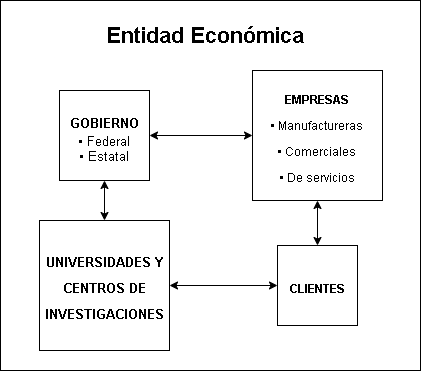
\includegraphics[width=12cm,height=4cm]{modeloo_moderno.drawio.png}
    \bigskip
    \\\small\textit{Nota}. Adaptado de \cite{tomta-2009}. %citar al tmta. 
    (Autoría Propia, s.f.)
\end{figure}
\vspace{\baselineskip}
En ámba definiciones,\begin{justifying}
     el modelo simplificado de cadena es mostrado en la Figura 2.
\end{justifying}
\begin{figure}[H]
    \caption{\emph{Modelo moderno de una cadena productiva\\}}
    \centering
    \smallskip
    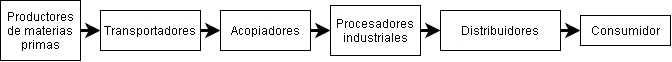
\includegraphics[width=16cm,height=2cm]{cadena.png}
    \bigskip
    \\\small\textit{Nota}. Adaptado de \cite{castro-2005}. %citar al castro. 
    (Autoría Propia, s.f.)
\end{figure}
\vspace{\baselineskip}
\subsubsection{Ejemplo: Bitcoin}
Uno de \begin{justifying}
    los ejemplos más prominentes de cadenas productivas es aquel de la primer criptomoneda el mundo, Bitcoin. 
    Acorde al \emph{whitepaper} \citep{article}, %citar al satoshi nakamoto
        Bitcoin es una propuesta para resolver el problema del doble gasto sin necesidad de un intermediario de confianza por medio
        de firmas digitales con estámpas de tiempo hasheadas en la red que forman un registro que no puede cambiarse a menos que se redefina
        dicha solución; estas firmas se auditoran por medio de nodos que mantienen una copia de todas las transacciones confirmadas por la red que se apodan
        la \emph{blockchain} (\emph{cadena de bloques} por su traducción al español).\par
\end{justifying}
Tomando \begin{justifying}
     el concepto de las cadenas productivas, Bitcoin 
    (como se muestra en la Figura 3) forma una cadena productiva moderna donde los mineros son los productores de la materia prima (bloques hash), transportan dicho
    bien para que pueda ser confirmado por el resto de la red, acaparan el bién en el caso de que la minería sea para ganancia propia, o lo terminan
    vendiendo por otro bien; si es el papel moneda, las casas de intercambio legalmente reguladas tendrán que brindar el papel moneda auditorado poro las instituciones fiscales vigentes. 
    En toda la cadena, el consumidor que adquiere la criptomoneda termina siendo registrado en la \emph{blockchain}
    para que futuras transacciones puedan confirmarse por la naturaleza computacional del protocolo.\par
\end{justifying}
\begin{figure}[H]
    \caption{\emph{Cadena productiva del protocolo Bitcoin\\}}
    \centering
    \smallskip
    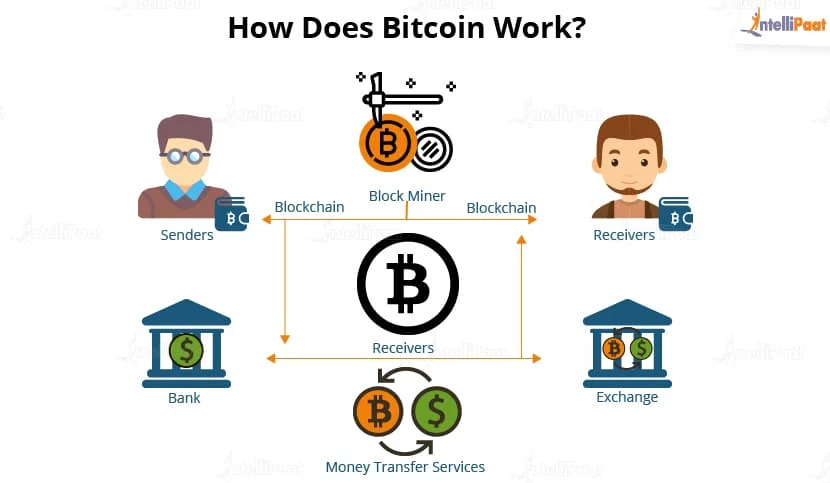
\includegraphics[width=14cm,height=8cm]{bitcoin.jpg}
    \bigskip
    \\\small\textit{Nota}. El diagrama en cuestión es una simplificación del funcionamiento de la red Bitcoin. \citep{intellipaat-2019}. %citar al intellipaat 
\end{figure}
\vspace{\baselineskip}
\section*{Conclusión}
Los \begin{justifying}
    estudios económicos tanto como sus cadenas productivas permiten al Desarrollo Sustentable entender los mecanismos que interfieren
    en la maquina económica que se estudie, ya sea las criptomonedas como las cadenas de suministro agricultoras. Con ello, podemos considerar
    alternativas tanto físicas como digitales para las economías que deseen integrar los principios del Desarrollo Sustentable, como las fuentes de energía renovables.\par
\end{justifying}
\newpage
% Referencias
\setcounter{secnumdepth}{0} %permite enumerar las secciones QUITAR SI QUIERES OG APA7
\renewcommand\refname{\textbf{Referencias}}
\bibliography{referencias} %el archivo 'referencias.bib' debe estar dentro del mismo folder donde se encuentra el archivo .tex para citar las referencias deseadas

\end{document}